\documentclass[10pt,a4paper]{article}
\usepackage{CJKutf8}
\renewcommand{\tablename}{表}
\usepackage{geometry}
\usepackage{graphicx}
\usepackage{float}
\usepackage{multicol}
\usepackage{multirow}
\usepackage{xcolor}
\usepackage[colorlinks]{hyperref}
\usepackage{caption}
\definecolor{grey}{rgb}{0.8,0.8,0.8}
\definecolor{darkgreen}{rgb}{0,0.3,0}
\definecolor{darkblue}{rgb}{0,0,0.3}
\usepackage{enumitem}
\usepackage{tcolorbox}
\tcbuselibrary{skins,breakable,raster,listingsutf8}
\lstset{language=[x86masm]Assembler}
\newtcbinputlisting{code}[3]{colframe=yellow!30!black,listing options={showstringspaces=false,
		showspaces=false,%
		tabsize=2,%
		basicstyle={\ttfamily\normalsize},%
		keywordstyle=\color{blue!80!black}\bfseries,%
		identifierstyle=,%
		commentstyle=\color{green!50!blue}\itshape,%
		stringstyle=\color{green!50!black},%
		rulesepcolor=\color{gray!20!white},
		breaklines,
		columns=flexible,
		extendedchars=false},listing file={code/#1},title={\textbf{#2}\\\small #3},listing only, breakable}
\usepackage{array}
\tcbset{fonttitle=\bfseries,breakable,
	colback=white,
	every box/.style={enhanced,
		before=\par\smallskip,after=\par\smallskip},
	every box on layer 2/.style={reset,every box,colback=yellow!10!white,
		drop fuzzy shadow}}
\geometry{left=1cm,right=1cm,top=1cm,bottom=1.5cm}
\graphicspath{{img/}}
%\def\img#1#2{\begin{figure}[htb]\centering\includegraphics[width=0.7\columnwidth]{img/#1.png}\caption{#2}\label{fig:#1}\end{figure}}
\def\img#1#2{\begin{tcolorbox}[title=#2]\includegraphics[width=\textwidth]{#1.png}\end{tcolorbox}}
\def\pdf#1#2{\begin{tcolorbox}[title=#2]\includegraphics[width=\textwidth]{#1.pdf}\end{tcolorbox}}
\setlist{nosep}
\begin{document}
	\begin{CJK}{UTF8}{song}
	\title{计算机组成}
	\date{}
	\begin{multicols}{3}
		\maketitle
		\section{微机}
		\textbf{微机结构}
\begin{itemize}
	\item Input 输入
	\item Output 输出
	\item Memory 存储器
	\item ALU 算术逻辑单元
	\item Control unit 控制单元
\end{itemize}

\begin{table*}
	\centering
	\caption{微机概念差异}
\begin{tabular}{|>{\bfseries}l|p{8cm}|}
	\hline
	微处理器 Microprocessor & 可以被微缩成集成电路规模的CPU电路,包含ALU,CU,寄存器 \\
	\hline
	微型计算机 Mircrocomputer & 微处理器,存储器,I/O,总线 \\
	\hline
	微型计算机系统 Microcomputer system & 以微型计算机为主体,配上I/O及系统软件就构成了微型计算机系统。 \\
	\hline
	微控制器 Microcontrollers & A microcontroller has a CPU in addition to a fixed amount of RAM, ROM, I/O ports on one single chip (\emph{e.g.} Cortex) \\
	\hline
	嵌入式系统 Embedded Systems & An embedded system uses a microcontroller or a microprocessor to do one task and one task only\\
	\hline
\end{tabular}
\end{table*}

\textbf{指令集}:CISC(1-n个字),RISC(1个字)

\textbf{字}:CPU一次可以处理的最大比特数

\textbf{位扩展}:同一地址的位扩展,满足一个字的输出

\textbf{字扩展}:增大字的量,选择不同的字,满足存储量需求

\begin{table*}
	\begin{minipage}{0.3\textwidth}
		\centering
		\caption{总线类型}
		\begin{tabular}{|c|c|c|}
			\hline
			\bfseries 类型 &\bfseries 仲裁 &\bfseries 时序 \\
			\hline
			单工 & 集中式 & 同步 \\
			多工 & 分布式 & 异步 \\
			\hline
		\end{tabular}
	\end{minipage}
	\begin{minipage}{0.7\textwidth}
		\centering
		\caption{总线结构}
		\begin{tabular}{|>{\bfseries}c|l|l|}
			\hline
			& \bfseries 优点 &\bfseries 缺点 \\
			\hline
			单线结构 & 简单 & 吞吐量低 \\
			\hline
			CPU-Central 双线结构 & 数据传输率高 & I/O与内存需要经过CPU \\
			\hline
			Memory-Central 双线结构 & CPU性能好 吞吐量高 &  \\
			\hline
		\end{tabular}
	\end{minipage}
\end{table*}


		\section{存储与I/O}
		\textbf{内存特征}
\begin{description}
	\item[Location]CPU,内部,外部
	\item[Capacity]字大小,字数目
	\item[Unit of transfer]内部(一字),外部(多字) --- Addressable Unit: 内部(一字节),外部(簇)
	\item[Access method] 访存方式
		\begin{itemize}
			\item Sequential 串行访问 (tape)
			\item Direct 直接访问 (disk)
			\item Random 随机访问 (RAM,ROM)
			\item Associative 关联访问 (cache)
		\end{itemize}
	\item[Performance] 评价指标
		\begin{itemize}
			\item Access time
			\item Memory Cycle time
			\item Transfer Rate
		\end{itemize}
	\item[Physical type] 物理类型
		\begin{itemize}
			\item Semiconductor (RAM)
			\item Magnetic (disk \& tape)
			\item Optical (CD \& DVD)
			\item Others (Bubble Hologram)
		\end{itemize}
	\item[Organisation] Physical arrangement of bits into words(存储字)
\end{description}

\begin{table*}
	\begin{minipage}[b]{.5\linewidth}
	\centering
	\caption{RAM 区别}
	\begin{tabular}{|>{\bfseries}l|c|c|}
		\hline
		& \bfseries DRAM &\bfseries SRAM \\
		\hline
		字节存储方式 & 电容电荷 & 开关状态 \\
		电荷泄漏 & 有 & 无 \\
		刷新 & 需要 & 不需要 \\
		构造 & 简单 & 复杂 \\
		每位规模 & 更小 & 更大 \\
		价格 & 便宜 & 昂贵 \\
		刷新电路 & 需要 & 不需要 \\
		速度 & 更慢 & 更快 \\
		用途 & 主存储器 & 高速缓存 \\
		\hline
	\end{tabular}
	\end{minipage}
	\begin{minipage}[b]{.5\linewidth}
	\centering
	\caption{ROM 区别}
	\begin{tabular}{|>{\bfseries}p{10em}|p{8em}|}
		\hline
		掩膜型 ROM & 无法修改 \\
		\hline
		可编程只读存储器 PROM & 一旦写入,不可改变 \\
		\hline
		可擦除可编程只读存储器 EPROM & 可写,用紫外光擦除,重新写入 \\
		\hline
		点可擦除的可编程只读存储器 EEPROM & 通电擦除,重新写入 \\
		\hline
		闪存 Flash & 对芯片编程,通电擦除再写入 \\
		\hline
	\end{tabular}
	\end{minipage}
\end{table*}

\textbf{I/O数据传送方式}
\begin{description}
	\item[程序控制方式 Programmed I/O] CPU与外设之间的数据传送是在程序控制下完成的。用查询方式使 CPU 与外设交换数据时,CPU要不断读取状态位,检查输入设备是否已准备好数据。由于许多外设的速度很低,这种等待过程会占去CPU的绝大部分时间,而真正用于传输数据的时间却很少,使CPU的利用率变得很低。
	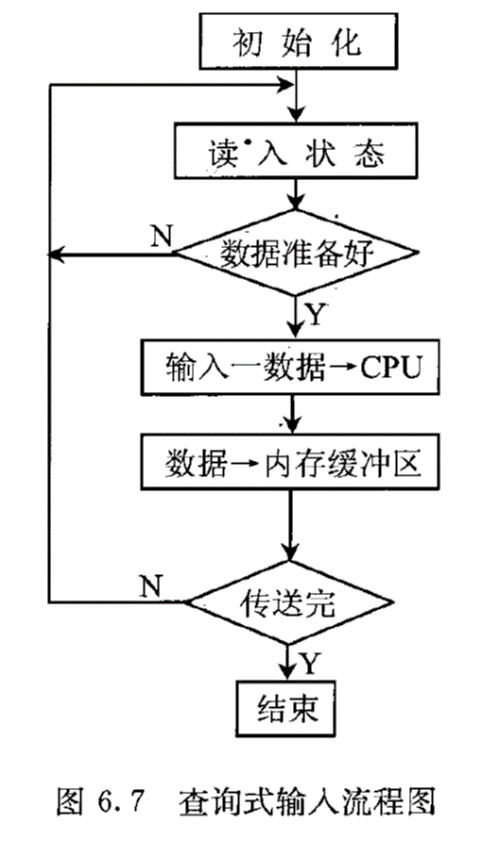
\includegraphics[width=0.75\columnwidth]{pinput.png}
	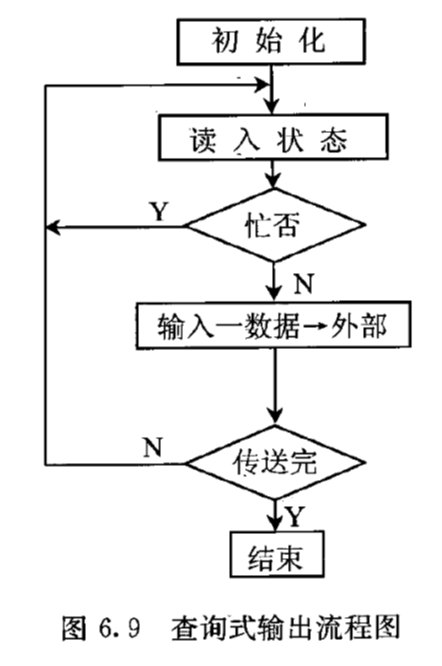
\includegraphics[width=0.75\columnwidth]{poutput.png}
	\item[中断方式 Interrupt driven I/O]采用中断方式后,CPU平时可以执行主程序,只有当输入设备将数据准备好了,或者输出端口的数据缓冲器已空时,才向CPU发中断请求。CPU响应中断后,暂停执行当前的程序,转去执行管理外设的中断服务程序(ISR)。在中断服务程序中,用于输入或输出指令在CPU和外设之间进行一次数据交换。等输入或输出操作完成之后,CPU又回去执行原来的程序。
	\begin{figure}[H]
	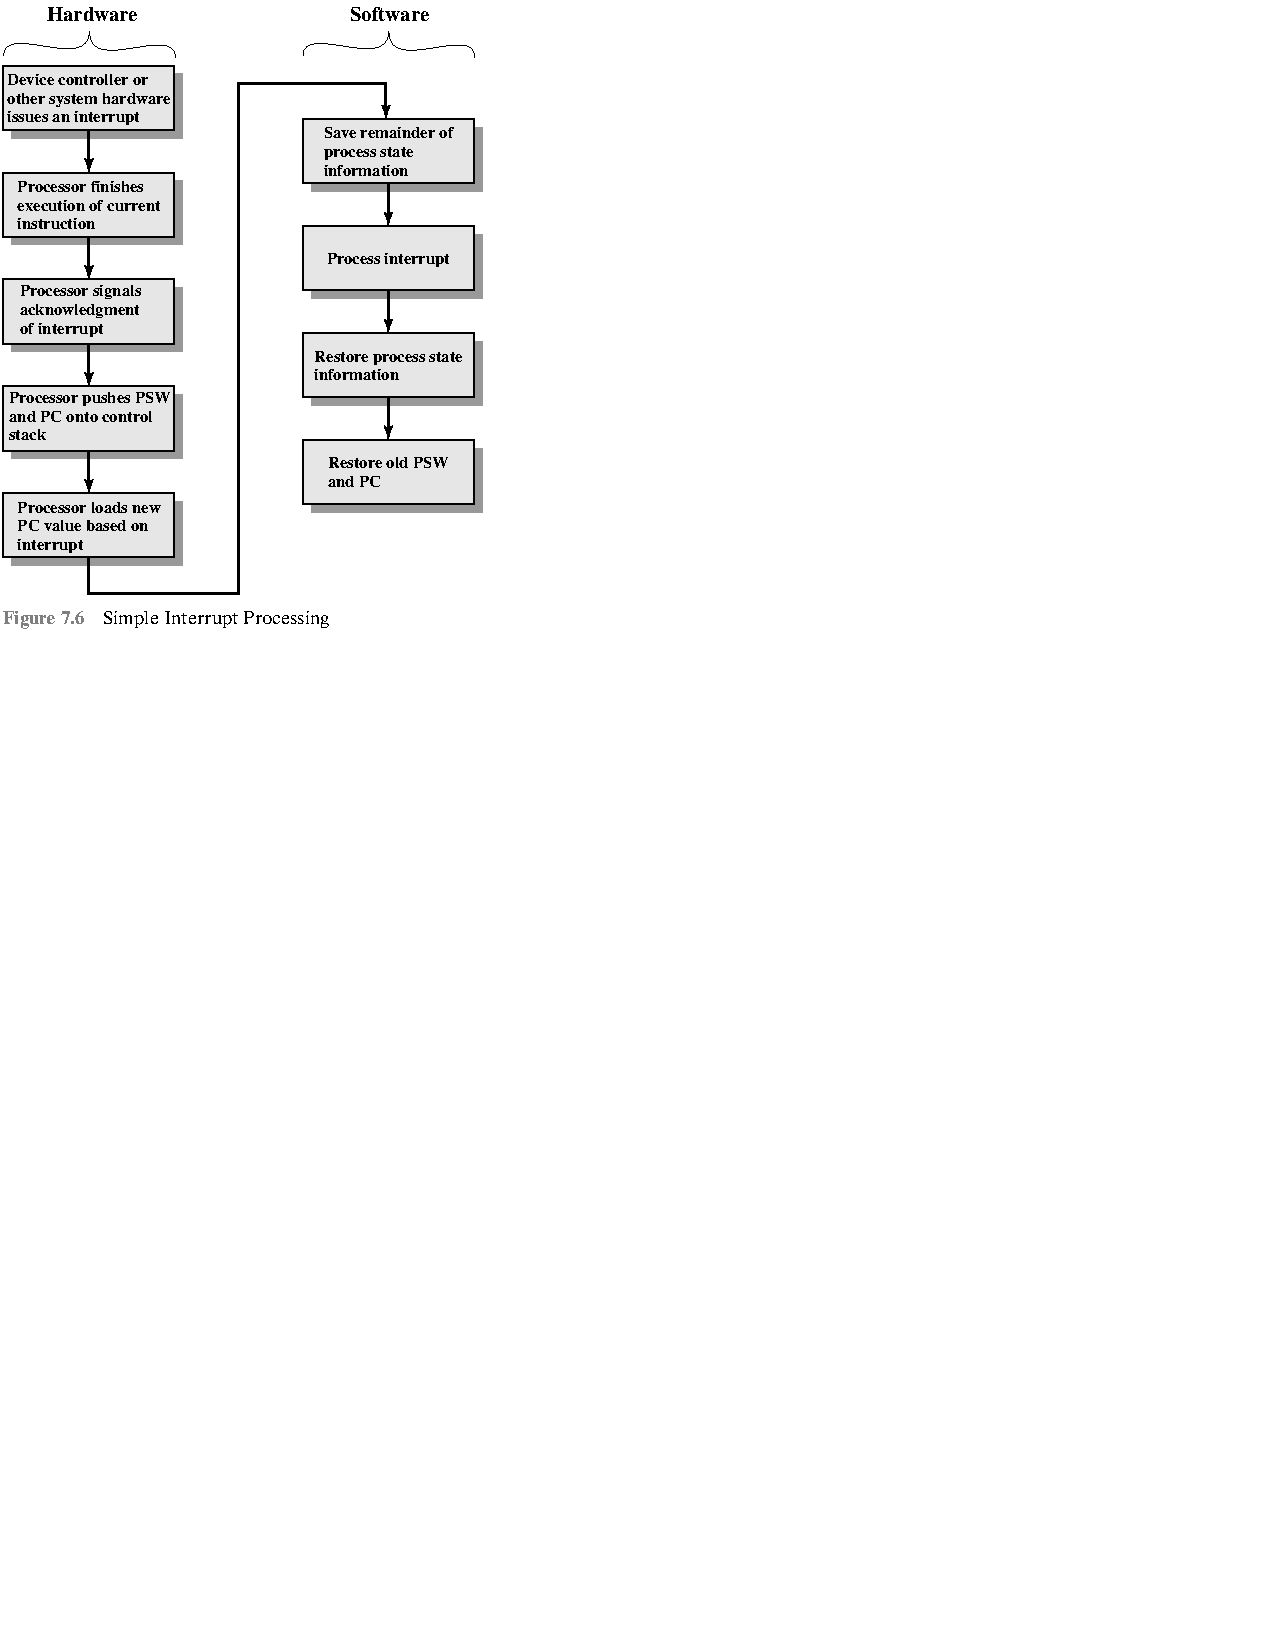
\includegraphics[width=\columnwidth]{interio.pdf}
	\end{figure}
	\item[直接存储器访问 DMA] DMA控制器临时接管总线,控制外设和存储器之间进行高速的数据传送,快速完成交换一批数据的任务,而不要CPU进行干预。这种控制器能给访问内存所需要的地址信息,并且能够自动修改地址指针,也能够设定和修改传送的字节数,还能够向存储器和外设发出相应的读写控制信号。在DMA传送结束后,它能够释放总线,把对总线的控制权又交还给CPU。
	\begin{figure}[H]
	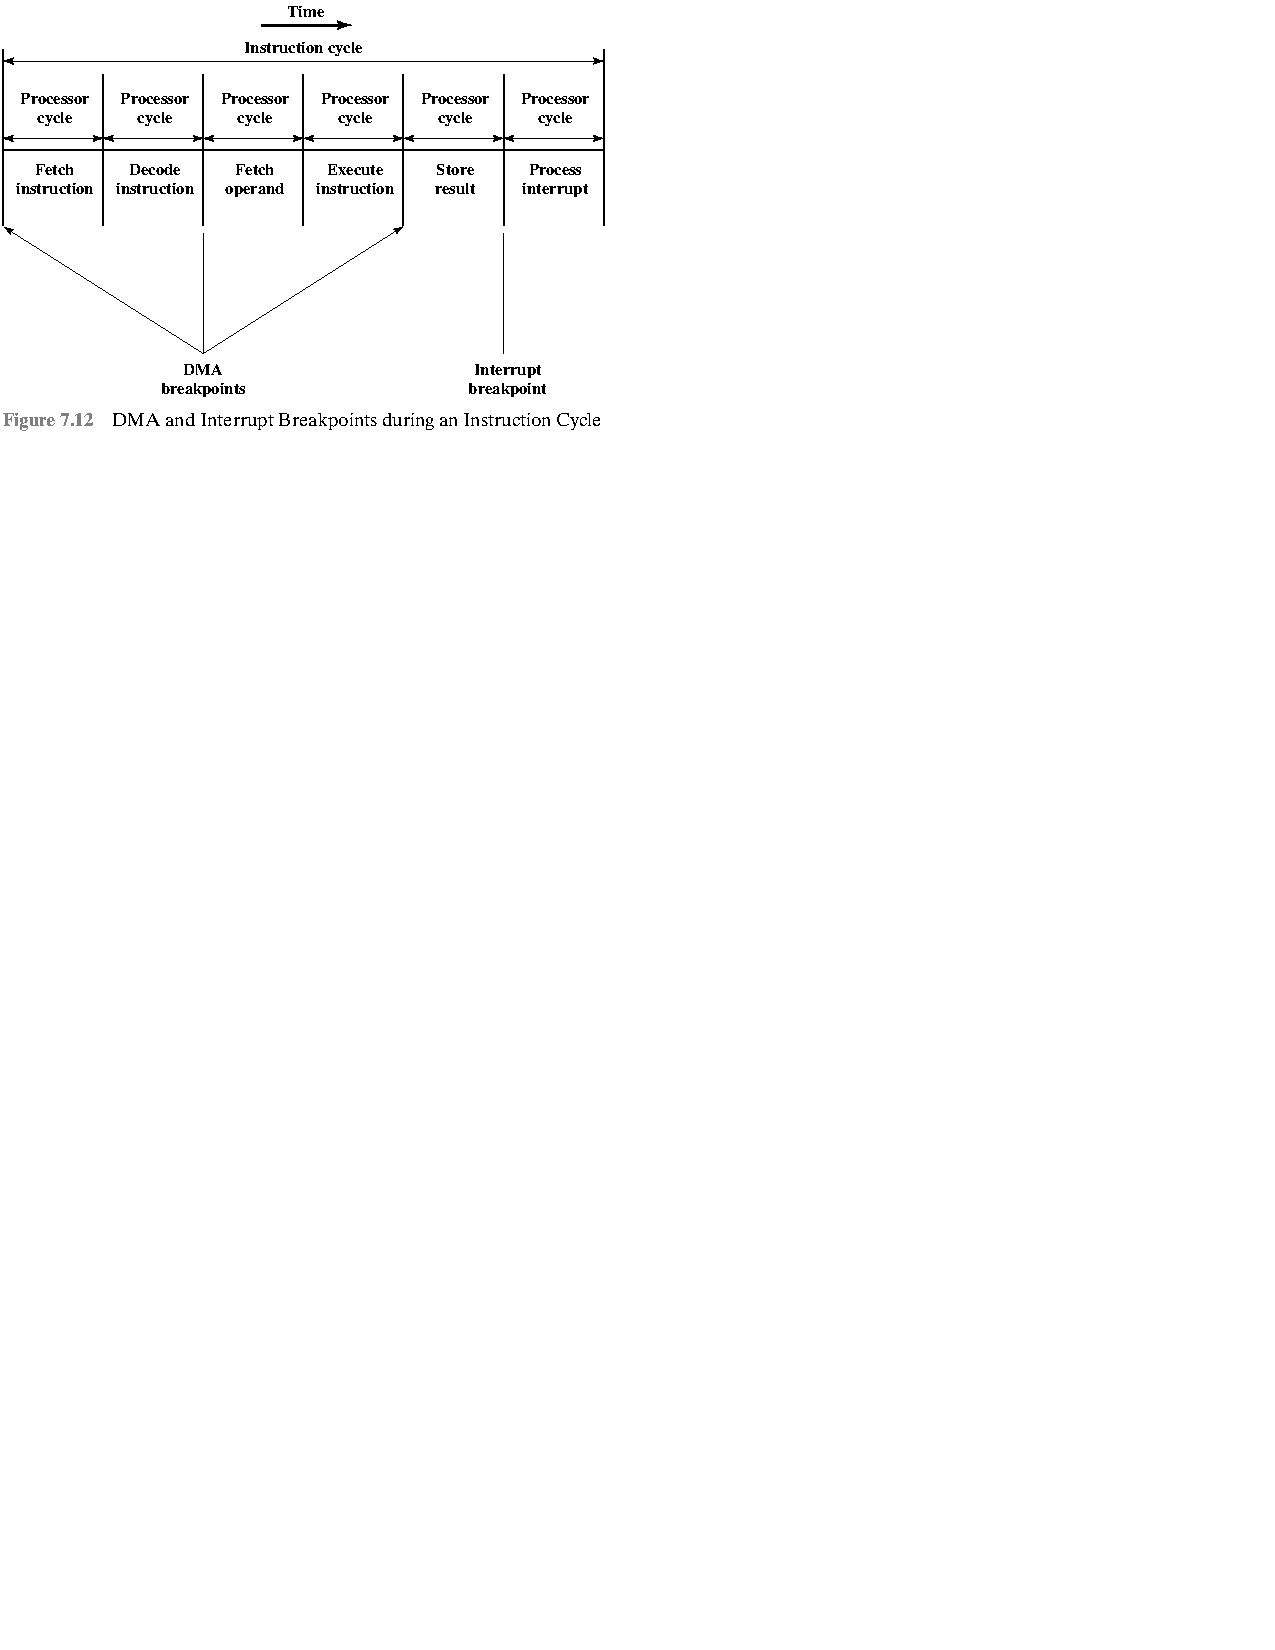
\includegraphics[width=\columnwidth]{DMA.pdf}
	\end{figure}
\end{description}

\begin{table*}
	\centering
	\caption{DMA 架构}
	\begin{tabular}{|>{\bfseries}l|c|c|}
		\hline
		& \bfseries 使用总线次数 &\bfseries CPU暂停次数 \\
		\hline
		Single Bus, Detached & 2 & 2 \\
		Single Bus,Intergrated & 1 & 1 \\
		Seperate I/O & 1 & 1 \\
		\hline
	\end{tabular}
\end{table*}

		\section{80x86}
		%\documentclass[10pt,a4paper]{article}
\usepackage{CJKutf8}
\renewcommand{\tablename}{表}
\usepackage{geometry}
\usepackage{graphicx}
\usepackage{float}
\usepackage{multicol}
%\usepackage{tcolorbox}
%\tcbuselibrary{skins,breakable,raster}
\usepackage{array}
%\tcbset{fonttitle=\bfseries,breakable,
%	colback=white,
%	every box/.style={enhanced,
%		before=\par\smallskip,after=\par\smallskip},
%	every box on layer 2/.style={reset,every box,colback=yellow!10!white,
%		drop fuzzy shadow}}

\geometry{left=1cm,right=1cm,top=1cm,bottom=1.5cm}
%\graphicspath{{img/}}
%\def\img#1#2{\begin{figure}[htb]\centering\includegraphics[width=0.7\columnwidth]{img/#1.png}\caption{#2}\label{fig:#1}\end{figure}}
\def\img#1#2{\begin{tcolorbox}[title=#2]\includegraphics[width=\textwidth]{#1.png}\end{tcolorbox}}
\def\pdf#1#2{\begin{tcolorbox}[title=#2]\includegraphics[width=\textwidth]{#1.pdf}\end{tcolorbox}}
\usepackage{enumitem}
\setlist{nosep}
\begin{document}
	\begin{CJK}{UTF8}{gbsn}
	\title{计算机组成}
	\date{}
%	\begin{multicols}{3}
\begin{description}
\item[8086] 16-bit, 20-bit address.
\item[8088] 16-bit internal, 8-bit external.
\end{description}

只有两段:
\begin{description}
	\item[BIU](Bus Interface Unit) 连接内存与外设。
	\item[EU](Execution Unit) 执行之前获取的指令。
\end{description}

\begin{table*}
	\centering
	\caption{8086 寄存器}
	\begin{tabular}{|>{\bfseries}l|c|l|}
		\hline
		Category & \bfseries Bits &\bfseries Register Names \\
		\hline
		General & 16 & \texttt{AX}(Accumulator), \texttt{BX}(Base), \texttt{CX}(Count), \texttt{DX}(Data) \\
		\hline
		& 8 & \texttt{AH}, \texttt{AL}, \texttt{BH}, \texttt{BL}, \texttt{CH}, \texttt{CL}, \texttt{DH}, \texttt{DL} \\
		\hline
		Pointer & 16 & \texttt{SP}(Stack Pointer), \texttt{BP}(Base Pointer) \\
		\hline
		Segment & 16 & \texttt{CS}(Code Segment), \texttt{DS}(Data Segment), \texttt{SS}(Stack Segment), \texttt{ES}(Extra Segment) \\
		\hline
		Instruction & 16 & \texttt{IP}(Instruction Pointer) \\
		\hline
		Flag & 16 & \texttt{FR}(Flag Register) \\
		\hline
	\end{tabular}
	\caption{段偏移寄存器}
	\begin{tabular}{|>{\bfseries}c|>{\ttfamily}c|>{\ttfamily}c|>{\ttfamily}c|>{\ttfamily}c|}
		\hline
		Segment register & CS & DS & ES & SS \\
		\hline
		Offset register & IP & SI,DI,BX & SI,DI,BX & SP,BP \\
		\hline
	\end{tabular}
	
\end{table*}

双工作模式
\begin{description}
	\item[最小模式] $\rm MN/\overline{MX}=1$ 单 CPU。
	\item[最大模式] $\rm MN/\overline{MX}=0$ 多 CPU(8086+8087),8288控制芯片。 
\end{description}

\begin{table*}
	\centering
	\caption{8086 接脚}
	\begin{tabular}{|>{\ttfamily}c|p{13em}|c|c|}
		\hline
		\bfseries Signal &\bfseries Description &\ttfamily 0 &\ttfamily 1 \\
		\hline
		ALE & Address Latch Enabled &  & Latched  \\
		\hline
		$\tt \overline{BHE}$ & Bank High Enabled & $\rm AD_8\sim \rm AD_{15}$ Enabled & $\rm AD_8\sim\rm AD_{15}$ Disabled \\
		\hline
		$\tt DT/\overline{R}$ & direction of Data Transfer & sending data & receiving data \\
		\hline
		$\tt \overline{DEN}$ & Data transceiver ENabled & enabled & disabled \\
		\hline
		$\tt \overline{WR}$ & WRiting to Mem/IO & writing & \\
		\hline
		$\tt \overline{RD}$ & ReaDing from mem/IO & reading & \\
		\hline
		$\tt M/\overline{IO}$ & CPU accessing Memory / IO & IO & Memory \\
		\hline
		$\tt INTR$ & INTerrupt Request, maskable by clearing IF &  & Requesting \\
		\hline
		$\tt \overline{INTA}$ & INTerrupt Acknowledge &  & Acknowledge \\
		\hline
		$\tt NMI$ & Non-Maskable Interrupt, CPU is interrupted after finishing the current instruction; cannot be masked by software &  & will be interrupted \\
		\hline
		$\tt HOLD$ & HOLD the bus request &  & hold \\
		\hline
		HLDA & HoLD request acknowledge &  & hold req ack \\
		\hline
		$\tt \overline{TEST}$ & for debug & test &  \\
		\hline
		READY & mem/IO is READY for transfer &  & ready \\
		\hline
		RESET & reset the CPU, IP, DS, SS, ES and 6 inst in instruction queue are cleared &  & CS=\texttt{0FFFFH} \\
		\hline
	\end{tabular}
\end{table*}

%\begin{figure}[H]
%	\centering
%	\caption{8086/88 周期}
%	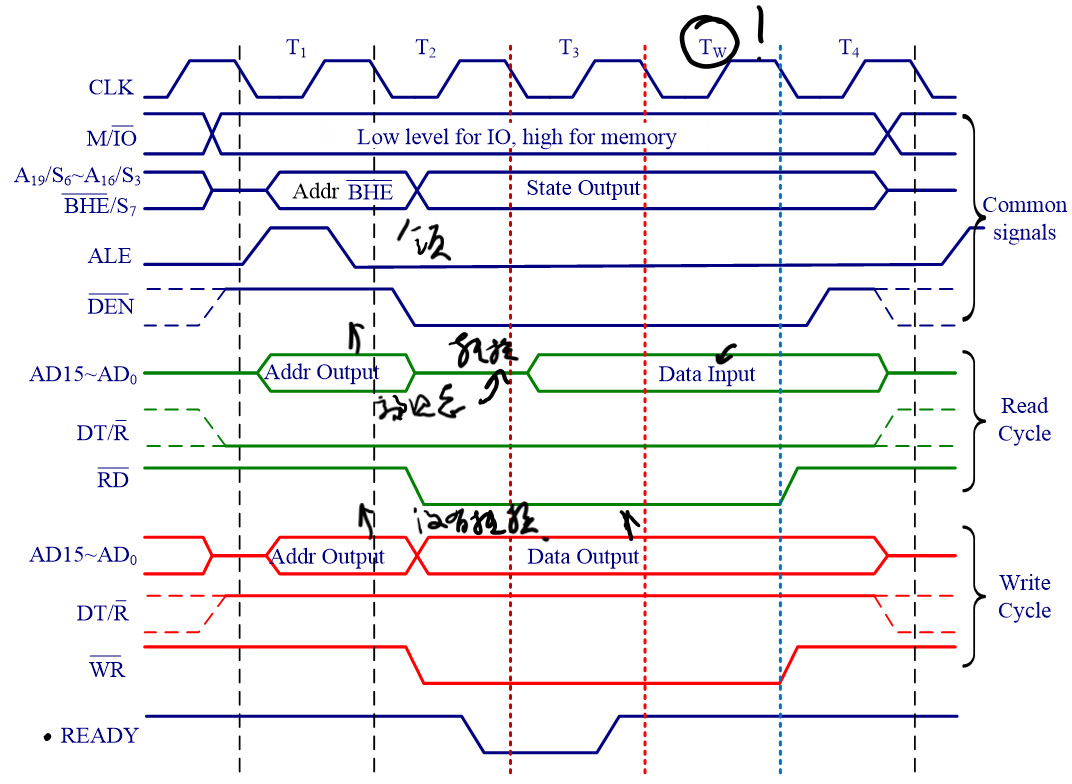
\includegraphics[width=\textwidth]{buscycle.png}
%\end{figure}
8086读周期时序:
在8086读周期内,有关总线信号的变化如下:
\begin{enumerate}
\item M/IO在整个读周期保持有效,当进行存储器读操作时,M/IO为高电平;当进行I/O端口读操作时,M/IO为低电平.
\item A19/S6~A16/S3是在T1期间,输出CPU要读取的存储单元的地址高4位.T2~T4期间输出状态信息S6~S3.
\item BHE/S7在T1期间输出BHE有效信号(BHE为低电平),表示高8位数据总线上的信息可以使用,BHE信号通常作为奇地址存储体的选择信号(偶地址存储体的选择信号是最低地址位A0).T2~T4期间输出高电平.
\item ADl5~AD0在T1期间输出CPU要读取的存储单元或I/O端口的地址A15~A0.T2期间为高阻态,T3~T4期间,存储单元或I/O端口将数据送上数据总线.CPU从ADl5~AD0上接收数据.
\item ALE:在T1期间地址锁存有效信号,为一正脉冲,系统中的地址锁存器正是利用该脉冲的下降沿来锁存A19/S6~A16/S3,ADl5~AD0中的20位地址信息以及BHE.
\item RD在T2期间输出低电平,送到被选中的存储器或I/O接口.要注意的是,只有被地址信号选中的存储单元或I/O端口,才会被RD信号从中读出数据(数据送上数据总线ADl5~AD0).
\item DT/R在整个总线周期内保持低电平,表示本总线周期为读周期.在接有数据总线收发器的系统中,用来控制数据传输的方向.
\item DEN在T2~T3期间输出有效低电平,表示数据有效.在接有数据总线收发器的系统中,用来实现数据的选通.
\end{enumerate}

8086写周期时序总线写操作的时序与读操作时序相似,其不同处在于:
\begin{enumerate}
\item 	
AD15~AD0在T2~T4期间送上欲输出的数据,而无高阻态.
\item WR在T2~T4期间输出有效低电平,该信号送到所有的存储器和I/O接口.要注意的是,只有被地址信号选中的存储单元或I/O端口才会被WR信号写入数据.
\item DT/R在整个总线周期内保持高电平,表示本总线周期为写周期.在接有数据总线收发器的系统中,用来控制数据传输方向.
\end{enumerate}

%%\end{multicols}
\end{CJK}
\end{document}
		\section{汇编}
		\begin{table}[H]
	\centering
	\caption{MODEL 大小}
	\begin{tabular}{|>{\ttfamily}c|c|c|}
		\hline
		.MODEL & code$\sim$64KB & data$\sim$64KB \\
		\hline
		SMALL & $>$& $\leq$ \\
		MEDIUM & $>$ & $\leq$ \\
		COMPACT & $\leq$ & $>$\\
		LARGE &$>$ &$><$ \\
		HUGE &$>$ &$>$ \\
		TINY &\multicolumn{2}{c|}{$<$} \\
		\hline
	\end{tabular}
\end{table}

\begin{table*}
	\begin{minipage}{0.6\textwidth}
		\centering
		\caption{PROC 范围}
		\begin{tabular}{|>{\ttfamily}c|c|c|}
			\hline
			PROC & IP & current code segment \\
			\hline
			SHORT & -128$\sim$127($\pm$1B) &  \\
			\hline
			NEAR & -32768$\sim$32767($\pm$2B) & within \\
			\hline
			FAR & changed along with CS & outside \\
			\hline
		\end{tabular}\\
		\raggedright
		\texttt{CALL} \textit{procedure}\\
		\raggedright\texttt{RET}\\
		\centering
		\caption{数据定义}
		\begin{tabular}{|>{\ttfamily}c|l|>{\ttfamily}l|}
			\hline
			&\bfseries 描述 &\bfseries 示例 \\
			\hline
			ORG & 指定开始偏移量 & ORG 10H \\
			\hline
			DB & 分配字节大小的块,依次写入 & Z DB "Good Morning" \\
			\hline
			EQU & 定义常量 & NUM EQU 234 \\
			\hline
			DUP & 复制字符 & x DB 6 DUP(23H) \\
			\hline
		\end{tabular}
	\end{minipage}
	\begin{minipage}{0.4\textwidth}
		\raggedright
		\texttt{CMP} op1,op2\\
		\centering
		\caption{跳转指令}
		\begin{tabular}{|>{\ttfamily}l|>{\ttfamily}l|c|}
			\hline
			Mnemonic & Condition & op1$\sim$op2 \\
			\hline
			\multicolumn{3}{|c|}{Signed} \\
			\hline
			JA/JNBE & CF=0 \& ZF=0 & $>$ \\
			JAE/JNB & CF=0 & $\geq$ \\
			JB/JNAE & CF=1 & $<$\\
			JBE/JNA & CF=1 | ZF=1 & $\leq$ \\
			\hline
			\multicolumn{3}{|c|}{Unsigned} \\
			\hline
			JG/JNLE & SF=OF \& ZF=0 & $>$ \\
			JGE/JNL & SF=OF &$\geq$ \\
			JL/JNGE & SF $\oplus$ OF & $<$\\
			JLE/JNG & ZF=1 | SF $\oplus$ OF & $\leq$ \\
			\hline
		\end{tabular}
	\end{minipage}
\end{table*}

\texttt{PTR} 可以暂时性更改一个变量的类型。
\begin{verbatim}
	DATA1  DB  10H,20H,30H  ;  
	DATA2  DW  4023H,0A845H 

	MOV  BX, WORD PTR DATA1	
	; 2010H -> BX
	MOV  AL, BYTE PTR DATA2	
	; 23H -> AL 
	MOV  WORD PTR [BX], 10H 
	; [BX],[BX+1] <- 0010H
	
	JMP FAR PTR aLabel
\end{verbatim}

8086 中没有内存到内存的直接运算。

除法运算比较特殊。

\begin{table}[H]
\begin{tabular}{|c|>{\ttfamily}c|>{\ttfamily}c|>{\ttfamily}c|>{\ttfamily}c|}
	\hline
	type & op1 & op2 & $\frac{\tt op1}{\tt op2}$ & mod \\
	\hline
	B/B & AL & src & AL & AH \\
	\hline
	W/W & AX & src & AX & DX \\
	\hline
	W/B & AX & src & AL & AH \\
	\hline
	DW/W & DX,AX & src & AX & DX \\
	\hline
\end{tabular}
\end{table}

跳转前的比较:\texttt{CMP dest,src}
\begin{table}[H]
	\centering
	\begin{tabular}{|>{\ttfamily}c|>{\ttfamily}c|>{\ttfamily}c|}
		\hline
		& CF & ZF \\
		\hline
		dest > src & 0 & 0 \\
		\hline
		dest = src & 0 & 1 \\
		\hline
		dest < src & 1 & 0 \\
		\hline
	\end{tabular}
\end{table}
不需要比较的跳转:
\begin{table}[H]
	\centering
	\begin{tabular}{|>{\ttfamily}l|>{\ttfamily}l|l|}
		\hline
		Mnemonic & Condition & 跳转条件 \\
		\hline
		JNC & CF=0 & 不进位 \\
		\hline
		JNE/JNZ & ZF=0 & 不等于0 \\
		\hline
		JNO & OF=0 & 没有溢出 \\
		\hline
		JNP/JPO & PF=0 & 奇校验 \\
		\hline
		JNS & SF=0 & 不是负数 \\
		\hline
		JP & OF=1 & 溢出 \\
		\hline
		JP/JPE & PF=1 & 偶校验 \\
		\hline
		JS & SF=1 & 负数 \\
		\hline
	\end{tabular}
\end{table}

\begin{table*}
	\begin{minipage}{0.5\textwidth}
	\centering
	\caption{算术运算}
	\begin{tabular}{|>{\ttfamily}c|>{\ttfamily}c|>{\ttfamily}c|>{\ttfamily}l|}
		\hline
		& op1 & ,op2 & calc \\
		\hline
		ADD & dest & src & dest = dest src \\
		\hline
		ADC & dest & src & dest = dest + src + CF \\
		\hline
		SUB & dest & src & dest = dest - src \\
		\hline
		SBB & dest & src & dest = dest - src - CF \\
		\hline
		INC & dest &  & dest = dest + 1 \\
		\hline
		DEC & dest &  & dest = dest -  1 \\
		\hline
		MUL & src &  & (DX,) AX = src * AX \\
		\hline
		DIV & src &  & AL = AL / src, AH = AL mod src* \\
		\hline
	\end{tabular}
	\end{minipage}
	\begin{minipage}{0.5\textwidth}
		\centering
		\caption{逻辑运算}
		\begin{tabular}{|>{\ttfamily}c|>{\ttfamily}c|>{\ttfamily}c|>{\ttfamily}l|}
			\hline
			& op1 & ,op2 & calc \\
			\hline
			AND & dest & src & dest = dest \& src \\
			\hline
			OR & dest & src & dest = dest | src \\
			\hline
			XOR & dest & src & dest = dest $\oplus$ src \\
			\hline
			NOT & dest &  & dest = $\sim$dest \\
			\hline
			SHR & dest & reg & dest = dest >> reg(zero-ext) \\
			\hline
			SHL & dest & reg & dest = dest << reg \\
			\hline
			ROL & dest & reg & dest = >> dest << reg \\
			\hline
			RCL & dest & reg & dest = >> CF << dest << reg \\
			\hline
		\end{tabular}
	\end{minipage}
\end{table*}
		\section{芯片}
		\subsection{存储器}
\paragraph{Checksum} 不进位地将所有的字节相加,取和的二的补码。
\paragraph{Parity bit} 考虑原有位和奇偶校验位1的个数的总和。偶校验:当序列中有奇数个1时设置为1;奇校验:当序列中有偶数个1时设置为1。
\paragraph{CRC} for disks and the Internet.
$k$-bit data, $n$-bit CRC:
\begin{equation}
	CRC = (M(X)\times X^n) \bmod G(X)
\end{equation}

\begin{table*}
	\centering
	\caption{存储器访问}
	\begin{tabular}{|>{\ttfamily}l|>{\ttfamily}c|>{\ttfamily}c|c|}
		\hline
		 & $\rm \overline{BHE}$ & A0 & 访问 \\
		\hline
		MOV AL, [100h] & 1 & 0 & D7-D0 \\
		\hline
		MOV AL, [101h] & 0 & 1 & D15-D8 \\
		\hline
		MOV AX, [100h] & 0 & 0 & D15-D0 \\
		\hline
		\multirow{2}{*}{MOV AX, [101h]} & 0 & 1 & D15-D8 \\
		\cline{2-4}
		& 1 & 0 & D7-D0 \\
		\hline
	\end{tabular}
\end{table*}

\subsection{外设 8255}

\begin{table*}
\begin{minipage}{0.4\textwidth}
	\centering
	\caption{8255 功能信号}
\begin{tabular}{|ccc|cc|c|}
	\hline
	$\rm \overline{CS}$ & $\rm A_1$ & $\rm A_0$ & $\rm \overline{RD}$ & $\rm \overline{WR}$ &\bfseries Function \\
	\hline
	0 & 0 & 0 & 0 & 1 & PA$\rightarrow$Data bus \\
	\hline
	0 & 0 & 1 & 0 & 1 & PB$\rightarrow$Data bus \\
	\hline
	0 & 1 & 0 & 0 & 1 & PC$\rightarrow$Data bus \\
	\hline
	0 & 0 & 0 & 1 & 0 & Data bus$\rightarrow$PA \\
	\hline
	0 & 0 & 1 & 1 & 0 & Data bus$\rightarrow$PB \\
	\hline
	0 & 1 & 0 & 1 & 0 & Data bus$\rightarrow$PC \\
	\hline
	0 & 1 & 1 & 1 & 0 & Data bus$\rightarrow$CR \\
	\hline
	1 &  &  & 1 & 1 & $\rm D_0 \sim D_7$ in float \\
	\hline
\end{tabular}
\end{minipage}
\begin{minipage}{0.6\textwidth}
	\centering
	\caption{8255 模式}
	\begin{tabular}{|c|c|c|c|c|}
		\hline
		&\bfseries Mode 0 &\bfseries Mode 1 &\bfseries Mode 2 &\bfseries BSR \\
		\hline\hline
		PCU & $\rm PC_7 \sim PC_4$ & $\rm PC_7 \sim PC_3$ & $\rm PC_7 \sim PC_3$&  \\
		\hline
		PCL &$\rm PC_3 \sim PC_0$&$\rm PC_2 \sim PC_0$&  &  \\
		\hline\hline
		PA & I/O & I/O & I\&O & I \\
		\hline
		PB & I/O & I/O &  & I \\
		\hline
		PCU & I/O & Handshake for PA & Handshake for PA &\multirow{2}{*}{O}\\
		\cline{1-4}
		PCL & I/O & Handshake for PB &  & \\
		\hline
	\end{tabular}
\end{minipage}

	\centering
	\caption{8255 模式字(CR)}
	\begin{tabular}{|>{\ttfamily}c|c|c|c|c|c|c|c|c|}
		\hline
		& D7 & D6 & D5 & D4 & D3 & D2 & D1 & D0 \\
		\hline\hline
		& 1 & Group A & Group A & PA & PCU & Group B & PB & PCL \\
		\hline
		0 &  &\multicolumn{2}{c|}{00 Mode 0 Simple I/O} & Output & Output & Mode 0 & Output & Output \\
		\hline
		1 & Input/Output modes & 1* Mode 2 & 01 Mode 1 & Input & Input & Mode  1 & Input & Input \\
		\hline\hline
		& 0 & * & * & * & PC & PC & PC & Set \\
		\hline
		0 & BSR mode &  &  &  &\multicolumn{3}{c|}{000 $\rm PC_0$} & Reset \\
		\hline
		1 &  &  &  &  & \multicolumn{3}{c|}{111 $\rm PC_7$} & Set \\
		\hline
	\end{tabular}
\end{table*}

\subsection{计时器 8253}

\begin{table*}
	\begin{minipage}{0.31\textwidth}
		\centering
		\caption{8253 功能信号}
		\begin{tabular}{|ccc|cc|p{5em}|}
			\hline
			$\rm \overline{CS}$ & $\rm A_1$ & $\rm A_0$ & $\rm \overline{RD}$ & $\rm \overline{WR}$ &\bfseries Function for counter\\
			\hline
			0 & 0 & 0 & 1 & 0 & W C0 \\
			\hline
			0 & 0 & 1 & 1 & 0 & W C1 \\
			\hline
			0 & 1 & 0 & 1 & 0 & W C2 \\
			\hline
			0 & 1 & 1 & 1 & 0 & W CP \\
			\hline
			0 & 0 & 0 & 0 & 1 & R C0 \\
			\hline
			0 & 0 & 1 & 0 & 1 & R C1 \\
			\hline
			0 & 1 & 0 & 0 & 1 & R C2 \\
			\hline
			0 & 1 & 1 & 0 & 1 & \textit{R CP (for 8254) }\\
			\hline
			1 &  &  & * & * & Not Available \\
			\hline
		\end{tabular}
	\end{minipage}
	\begin{minipage}{0.77\textwidth}
		\centering
		\caption{8253 模式}
		\begin{tabular}{|p{4em}|p{4em}|p{4em}|p{4em}|p{4em}|p{4em}|p{4em}|}
			\hline
			& Mode 0 & Mode 1 & Mode 2 & Mode 3 & Mode 4 & Mode 5 \\
			\hline
			& Interrupt on terminal count & One-shot & Rate-generator & Square wave rate-generator & Software triggered strobe & Hardware triggered strobe \\
			\hline
			initial & L & H & H & H & H & H \\
			\hline
			count started & L & L & H & H & H & H \\
			\hline
			Gate=1 & enable counting & pulse to retrigger & repeat counting & repeat counting & enable & pulse to retrigger \\
			\hline
			Gate=0 & disable counting & enable & disable counting & Output L$\rightarrow$H, disabled & disable & enable \\
			\hline
			Terminal & H & H & L & odd: H for $\frac{n+1}{2}$, L for $\frac{n-1}{2}$ & L$\rightarrow$H & L$\rightarrow$H \\
			\hline
		\end{tabular}
	\end{minipage}

\centering
\caption{8253 模式字}
\begin{tabular}{|c|c|c||c|c|c||c|c|c|c||c|c|}
	\hline
	D7 & D6 & & D5 & D4 & & D3 & D2 & D1 & & D0 & \\
	\hline
	SC1 & SC0 &  & RW1 & RW0 &  & M2 & M1 & M0 &  & BCD &  \\
	\hline
	0 & 0 & Select Counter 0 & 0 & 0 & Counter latch command & 0 & 0 & 0 & Mode 0 & 0 & 16-bit \\
	\hline
	0 & 1 & Select Counter 1 & 0 & 1 & R/W least byte & 0 & 0 & 1 & Mode 1 & 1 & BCD \\
	\hline
	1 & 0 & Select Counter 2 & 1 & 0 & R/W most byte & * & 1 & 0 & Mode 2 &  &  \\
	\hline
	1 & 1 & \textit{READ back for 8254 }& 1 & 1 & R/W least, then most & * & 1  & 1 & Mode 3 &  &  \\
	\hline
	&  &  &  &  &  & 1 & 0 & 0 & Mode 4 &  &  \\
	\hline
	&  &  &  &  &  & 1 & 0 & 1 & Mode 5 &  &  \\
	\hline
\end{tabular}
\end{table*}

\subsection{中断 8259}

8086/8088 有 256 个中断类型。
\begin{verbatim}
	INT 00H
	INT 0FFH
\end{verbatim}

中断向量表(IVT)
\begin{verbatim}
	CS = Type * 4
	IP = Type * 4 + 2
\end{verbatim}

中断服务程序(ISR)

\begin{table}[H]
	\begin{tabular}{|c|p{6em}|p{6em}|}
		\hline
		&\ttfamily CALL FAR &\ttfamily INT \\
		\hline
		jump & anywhere $\leq$ 1MB & a fix location \\
		\hline
		occurence & in the sequence of instructions & an external interrupt at any time \\
		\hline
		maskable & cannot be masked (disabled) & can be masked \\
		\hline
		save &\ttfamily CS:IP &\ttfamily FR+CS:IP \\
		\hline
		return  &\ttfamily RETF &\ttfamily IRET \\
		\hline
	\end{tabular}
\end{table}

中断优先级:
\begin{equation}\nonumber
	\rm	INT > NMI > INTR
\end{equation}

高优先级中断(数字小的)可以打断低优先级中断,低优先级中断只能在 EOI 之后才能够打断高优先级中断。
\begin{verbatim}
	STI	(EOI) IRET
\end{verbatim}

\subsection{连接 8251}
\begin{tabular}{|p{4em}|p{5em}|p{5em}|}
	\hline
	&\bfseries Parrallel &\bfseries Serial \\
	\hline
	transfer & 每一位用一条线 & 只用一条线 \\
	\hline
	bit & 一般用8条以上的线 & 线上每次传一位 \\
	\hline
	control signal & 需要额外的控制信号 & 不需要 \\
	\hline
	usage & 快速 昂贵 短距离 & 便宜 慢速 长距离 \\
	\hline
\end{tabular}
	\end{multicols}
	\begin{twocolumn}
%		\begin{multicols}{3}
%		\begin{tcbraster}[raster columns=3, raster equal height,
%			]
		\img{von}{冯诺依曼结构}
		\img{harvard}{哈佛结构}
		\img{struct}{微机结构}
		\img{sysstruct}{微机系统结构(哈佛结构)}
		\img{memhier}{内存层级}
		\img{memorg}{内存组织}
		\begin{tcolorbox}[title=总线结构]
		\img{singlebus}{单线结构}
		\img{dualbus}{CPU-Central 双线结构}
		\img{memdualbus}{Memory-Central 双线结构}
		\end{tcolorbox}
		\begin{tcolorbox}[title=寻址方式]
			\img{memio}{存储器映像寻址方式}
			\begin{tcolorbox}[title=I/O单独编址方式]
				\img{isoiod}{单工地址线}
				\img{isoiom}{多工地址线}
			\end{tcolorbox}
		\end{tcolorbox}
		\begin{tcolorbox}[title=RAM]
%			\begin{tcbraster}[raster columns=2,raster equal height=rows,]
%				\img{DRAM}{DRAM}
%				\img{SRAM}{SRAM}
%			\end{tcbraster}
			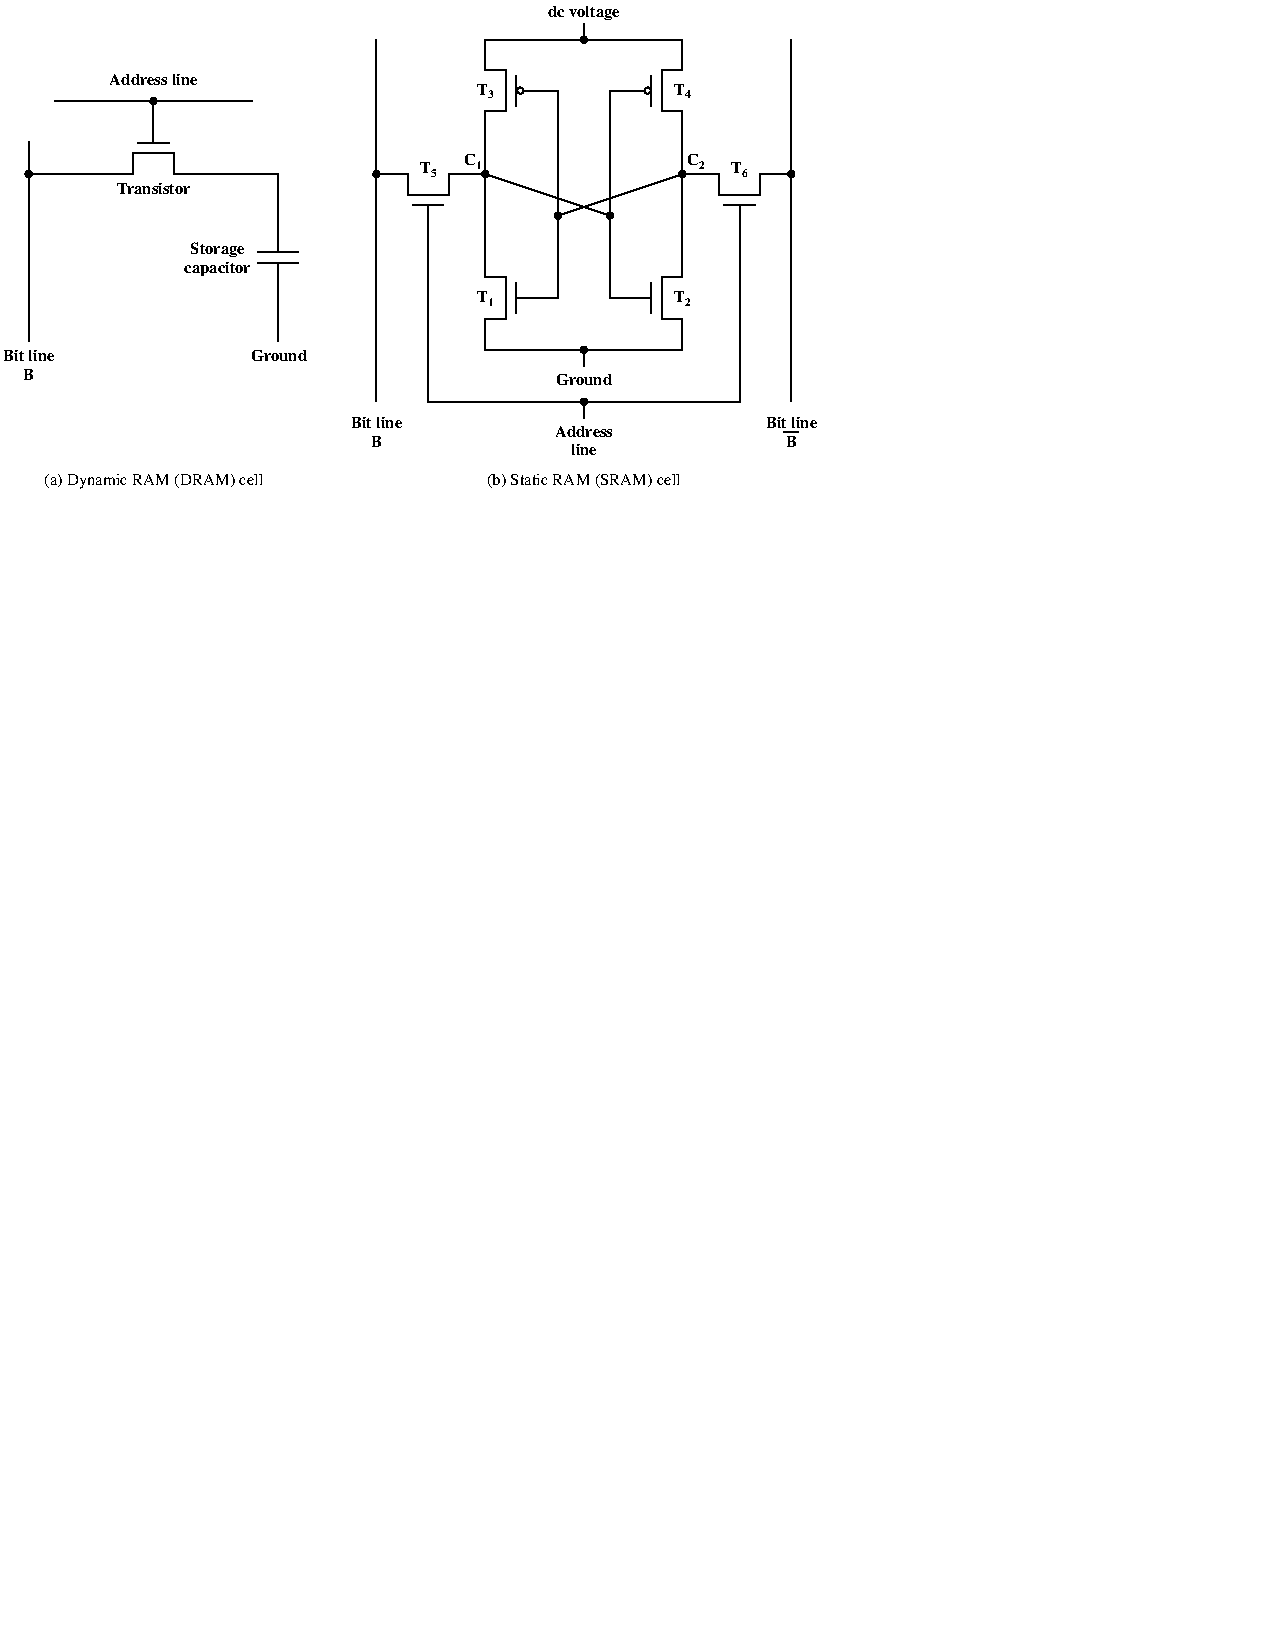
\includegraphics[width=\textwidth]{RAM.pdf}
		\end{tcolorbox}
		\pdf{DRAM16}{4M$\times$4 DRAM}
		\pdf{pkg}{存储芯片封装}
		\begin{tcolorbox}[title=存储位扩展]
			\pdf{bitext}{256K$\times$8-bit: 8 256$\times$1-bit}
			\img{bitext}{256K$\times$32-bit: 32 256K$\times$1-bit}
		\end{tcolorbox}
		\begin{tcolorbox}[title=存储字扩展]
			\pdf{wordext}{1M$\times$8-bit: 4 group 256K$\times$1-bit}
			\img{wordext}{2M$\times$8-bit: 8 group 256K$\times$8-bit}
		\end{tcolorbox}
		\begin{tcolorbox}[title=字与位同时扩展]
			\img{wbext}{32位可寻址单元}
			\img{wbextb}{1字节可寻址单元}
		\end{tcolorbox}
		\begin{tcolorbox}[title=外设]
			\centering
			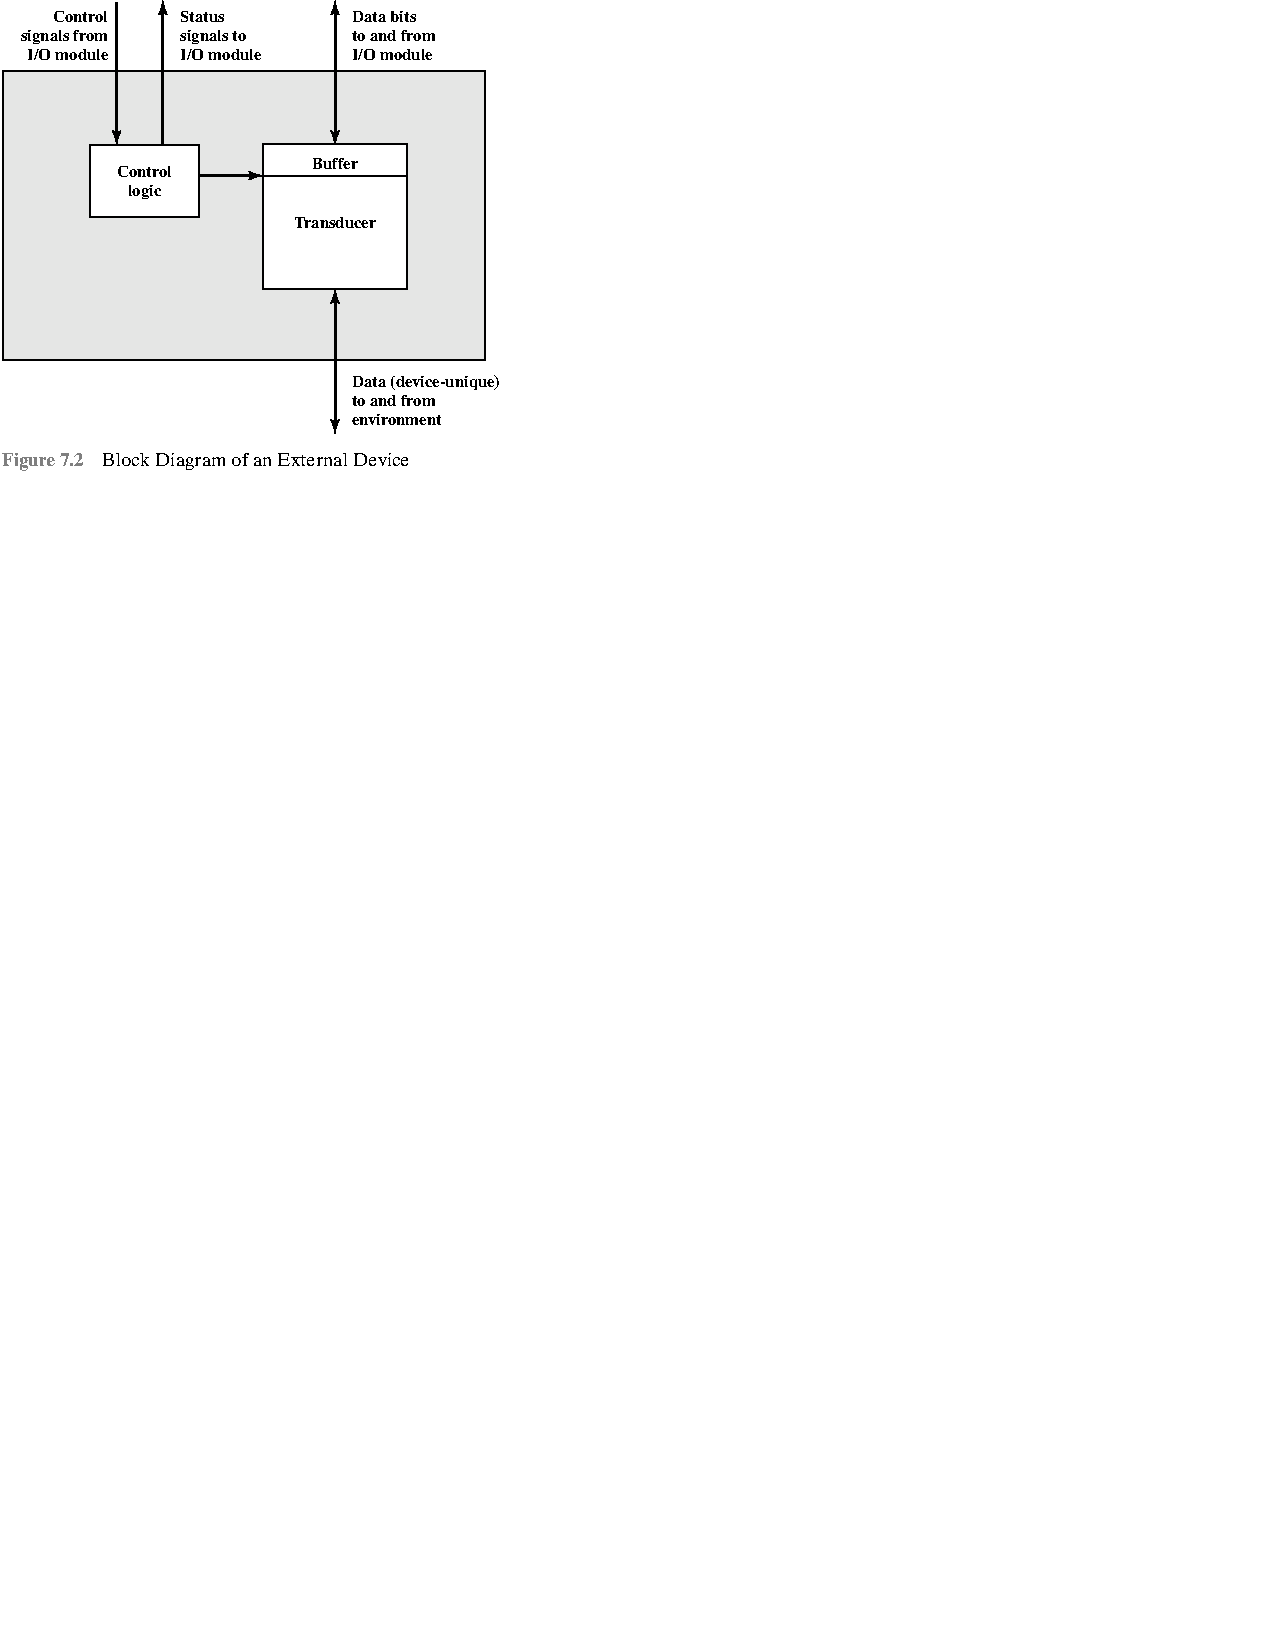
\includegraphics[width=0.7\linewidth]{pref.pdf}
		\end{tcolorbox}
		\pdf{iomod}{I/O模块}
		\pdf{interrupt}{中断处理内存变化}
		\pdf{DMAalter}{DMA架构}
		\img{8086}{8086内部结构}
		\img{8086l}{8086配置图}
		\begin{tcolorbox}[title=逻辑门电路]
			\centering
			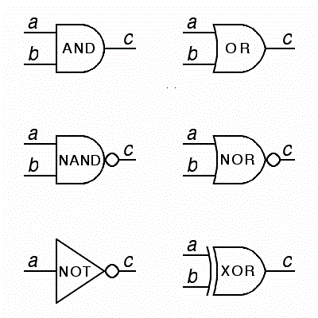
\includegraphics[width=0.75\textwidth]{CMOS.png}
%			\includegraphics[width=\textwidth]{logic.jpg}
			\begin{tabular}{|c|c|c|c|c|c|c|c|}
				\hline
				\multicolumn{2}{|c|}{input} & \multicolumn{6}{c|}{output} \\
				\hline
				$ a $ & $ b $  & $ ab $ & $ a+b $ & $ \overline{ab} $ & $ \overline{a+b} $& $\overline{a}$ & $a\oplus b$ \\
				\hline
				0 & 0 & 0 & 0 & 1 & 1 & 1 & 0 \\
				\hline
				0 & 1 & 0 & 1 & 1 & 0 & 1 & 1 \\
				\hline
				1 & 0 & 0 & 1 & 1 & 0 & 0 & 1 \\
				\hline
				1 & 1 & 1 & 1 & 0 & 0 & 0 & 0 \\
				\hline
			\end{tabular}
		\end{tcolorbox}
		\begin{tcolorbox}[title=锁存器和数据传输器]
			\img{latch}{74LS373 D Latch}
			\img{dt}{Data Bus Transceiver}
		\end{tcolorbox}
		\img{buscycle}{8086/88 总线周期}
		\begin{tcolorbox}[title=RAM\&ROM]
			\centering
%			\begin{tcolorbox}[title=RAM]
				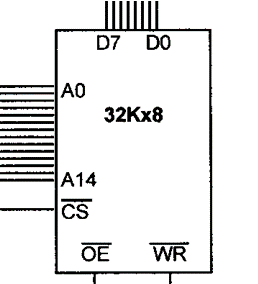
\includegraphics[width=0.3\textwidth]{RAMC.png}
%			\end{tcolorbox}
%			\begin{tcolorbox}[title=ROM]
				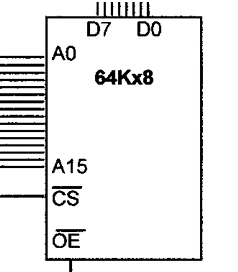
\includegraphics[width=0.3\textwidth]{ROMC.png}
%			\end{tcolorbox}
		\end{tcolorbox}
		\begin{tcolorbox}[title=74LS138 38译码器]
			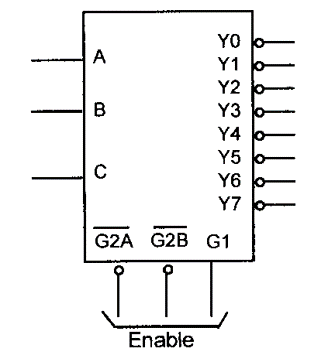
\includegraphics[height=4cm]{38G.png}
			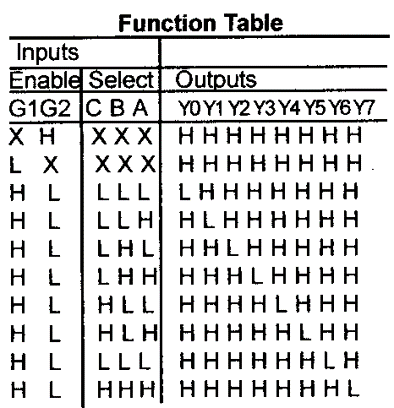
\includegraphics[height=4cm]{38T.png}
		\end{tcolorbox}
		\begin{tcolorbox}[title=8086存储组织]
			\centering
			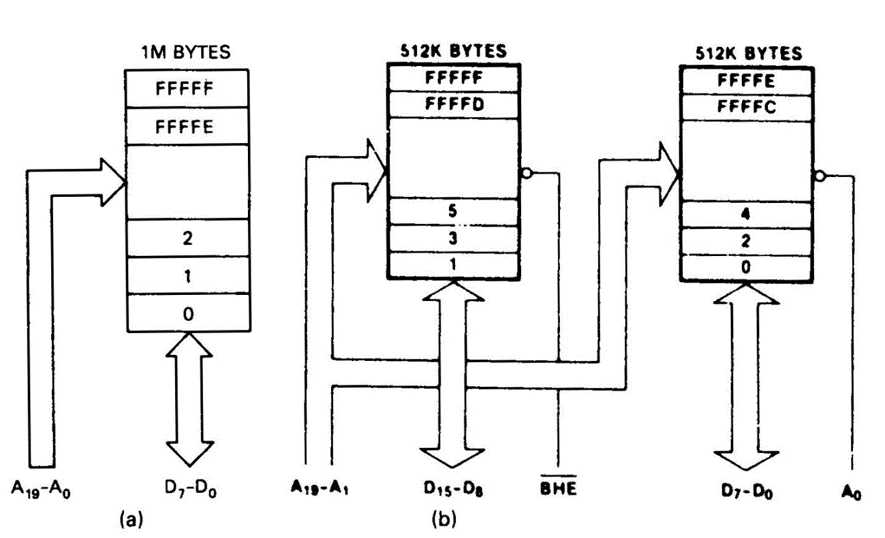
\includegraphics[width=\linewidth]{eobanks.png}
			\begin{tabular}{|c|c|c|c|}
				\hline
				$\rm \overline{BHE}$ & A0 &  &  \\
				\hline
				0 & 0 & Even word & D0-D15 \\
				\hline
				0 & 1 & Odd byte & D8-D15 \\
				\hline
				1 & 0 & Even byte & D0-D7 \\
				\hline
				1 & 1 & None &  \\
				\hline
			\end{tabular}
		\end{tcolorbox}
		\begin{tcolorbox}[title=8255 外设芯片]
			\centering
			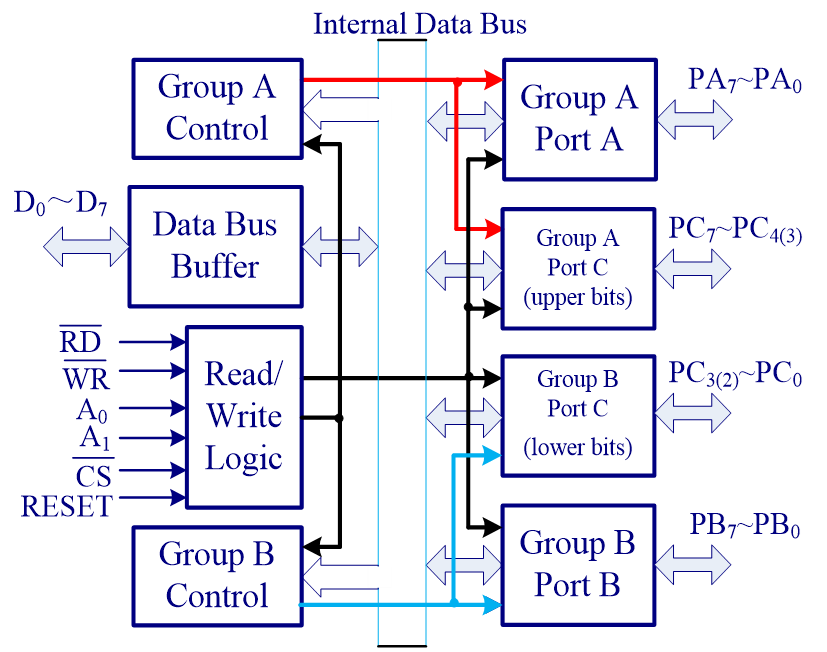
\includegraphics[width=0.7\linewidth]{8255.png}
		\end{tcolorbox}
		\begin{tcolorbox}[title=8253 计时器]
			\centering
			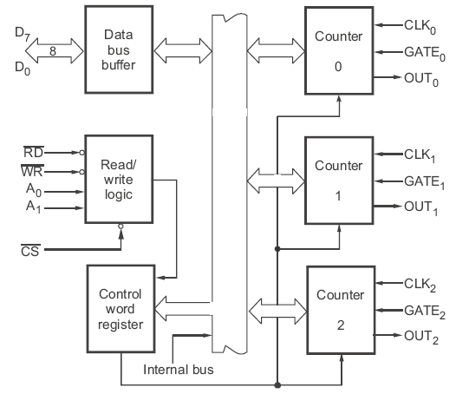
\includegraphics[width=0.7\linewidth]{8253.png}
		\end{tcolorbox}
		\begin{tcolorbox}[title=8253 计时器模式]
			\img{Mode0}{Mode 0---Interrupt on Terminal Count}
			\img{Mode1}{Mode 1---Hardware Retriggerable One-shot}
			\img{Mode2}{Mode 2---Rate Generator}
			\begin{tcolorbox}[title=Mode 3---Square Wave Rate Generator]
				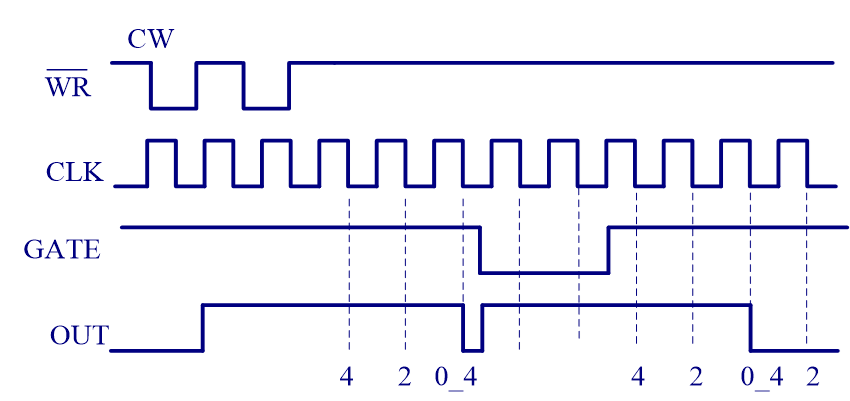
\includegraphics[width=\linewidth]{Mode3.png}
			\end{tcolorbox}
			\img{Mode4}{Mode 4---Software Triggered Strobe}
			\img{Mode5}{Mode 5---Hardware Triggered Strobe (Retriggerable)}
		\end{tcolorbox}
		\img{IVT}{8086/88 中断向量表}
		\begin{tcolorbox}[title=同步与异步]
			\begin{tabular}{|p{8em}|p{8em}|}
				\hline
				\bfseries 异步 &\bfseries 同步 \\
				\hline
				一次传一个字节 & 一次传一块数据 \\
				\hline
				使用start bit将接发者同步 & 使用 synch characters 将接发者同步 \\
				\hline
			\end{tabular}
			\img{async}{异步}
			\img{sync}{同步}
		\end{tcolorbox}
		\begin{tcolorbox}[title=8251 接口]
			\centering
			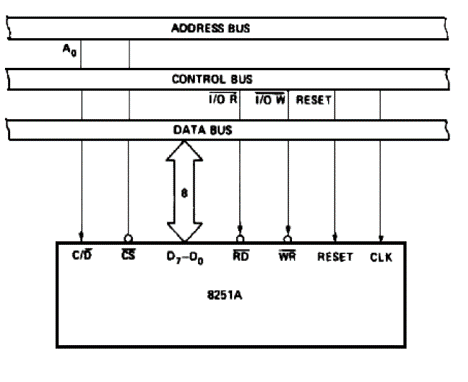
\includegraphics[width=0.7\linewidth]{8251.png}
			\begin{tabular}{|>{\ttfamily}c|>{\ttfamily}c|>{\ttfamily}c|>{\ttfamily}c|c|}
				\hline
				$\rm C/\overline{D}$ & $\rm\overline{RD}$ & $\rm\overline{WR}$ & $\rm\overline{CS}$ &\bfseries Function \\
				\hline
				0 & 0 & 1 & 0 & 8251 Data $\rightarrow$ data bus \\
				\hline
				0 & 1 & 0 & 0 & 8251 Bus $\rightarrow$ 8251 data \\
				\hline
				1 & 0 & 1 & 0 & status $\rightarrow$ data bus \\
				\hline
				1 & 1 & 0 & 0 & data bus $\rightarrow$ control \\
				\hline
				* & 1 & 1 & 0 & data bus $\rightarrow$ 3-state \\
				\hline
				* & * & * & 1 & data bus $\rightarrow$ 3-state \\
				\hline
			\end{tabular}
		\end{tcolorbox}
		\begin{tcolorbox}[title=8251 模式字]
			\img{8251async}{异步}
			\img{8251sync}{同步}
		\end{tcolorbox}
		\img{8251comm}{8251 命令字}
		\img{8251stat}{8251 状态字}
		\img{8251op}{8251 运转}
		\code{simpleio.asm}{实验一}{读取开关量状态取反后送显示}
%		\code{traffic.asm}{实验一}{交通灯}
		\code{converter.asm}{样例}{转换小写至大写}
		\code{banks.asm}{实验二}{奇偶存储奇偶数}
		\code{digit.asm}{样例}{输入送数码管显示}
		\code{8255.asm}{实验三}{8255送显示}
		\code{8253.asm}{实验三}{8253计时器}
		\code{IVT.asm}{实验三}{中断向量表(IVT)}
		\code{ISR.asm}{实验三}{中断服务程序(ISR)}
		Use 8251 to transfer 256 characters in async mode, assuming that the port addr are 208H and 209H, the baud factor is 16, and 1 stop bit, 1 start bit, no parity bit, and 8-bit character are used.
		\code{8251.asm}{样例}{8251 编程}
%		\end{tcbraster}
%		\end{multicols}
	\end{twocolumn}
	\end{CJK}
\end{document}